\documentclass[12pt]{article}

\usepackage{sbc-template}

\usepackage{graphicx,url}

\usepackage[portuguese]{babel}
\usepackage[utf8]{inputenc}  
\usepackage{hyperref}


     
\sloppy

\title{feather: Máquina de busca de entidades baseada na Wikipedia e Wikidata}

\author{Matheus C. Candido\inst{1}}


\address{Instituto de Ciências Exatas e Informática -- PUC Minas\\
Av Dom José Gaspar 500 -- 30.535-901 -- Belo Horizonte -- MG -- Brasil\\
\email{matheus.candido@sga.pucminas.br}
}

\begin{document} 

\maketitle
     
\begin{resumo} 
  Esse trabalho apresenta o desenvolvimento e os resultados de uma máquina de busca de entidades realizado para a disciplina de Recuperação de Informação. O \emph{dataset} utilizado é uma combinação dos \emph{dumps} da Wikipedia e Wikidata.

\end{resumo}

\section{Introdução}

Uma máquina de busca, \emph{search engine}, motor de busca ou qualquer uma dessas variações de nome, é um programa de computador responsável por retornar documentos relevantes para consultas de palavras-chave. Esses motores surgiram logo após o surgimento da Internet (WWW), como ferramenta trivial na vida dos usuários da rede.

Com o crescimento da WWW, muitos desses buscadores foram perdendo utilidade já que não estavam preparados para lidar com tamanho volume de dados. Foi necessário desenvolver técnicas aprimoradas em diversas áreas da Ciência da Computação como Recuperação de Informação e Computação Linguística para geração de técnicas de ranqueamento e índices invertidos eficientes, bem como nas áreas de Sistemas Distribuídos e Armazenamento para controlar a performance desses motores.

Uma máquina de busca aberta é aquela que é capaz de indexar todas as páginas de um determinado domínio, sem filtro algum, por exemplo. Os documentos desse tipo de máquina são geralmente dados não estruturados e de marcação HTML, sendo necessário pré-processamento e inteligência de máquina para selecionar o que é relevante ou não no documento. Máquinas de busca de entidades funcionam de maneira diferente. Cada documento dessas máquinas, é na verdade (mas não limitado) a representação de um objeto (de tipos pré-definidos ou não), como pessoas, locais, empresas ou acontecimentos. Esses dados são armazenados de forma estrutural e muitas vezes servem de conteúdo para bases de conhecimento.

A Wikidata é uma base de conhecimento aberta e serve como armazenamento central de dados estruturados de projetos da Wikimedia, como Wikipedia, Wikivoyage, Wikisource e outros. Para evitar replicação de armazenamento, já que os projetos geram terabytes de conteúdo anualmente, são gerados \emph{links} (ou ponteiros) para recursos nos projetos irmãos. Como os projetos mencionados em sua maioria são abertos (entradas podem ser editadas por qualquer pessoa), são oferecidos despejos de dados que podem ser gerados mensalmente ou semanalmente pela comunidade.

Nesse trabalho, exploramos a disponibilidade de tais despejos de dados (ou \emph{dumps}), com os seguintes objetivos:

\begin{itemize}
	\item Construir uma máquina de busca de entidades com resultados satisfatórios
	\item Agrupar diversos tipos de informações e metadados disponíveis nos despejos estruturais da Wikidata com os artigos publicados na Wikipedia
	\item Implementar uma interface de interação com usuário simples e minimalista, que contenha métricas para cada consulta
	\item Facilitar a comunicação com a máquina de buscas utilizando uma arquitetura RESTful
\end{itemize}


\section{Componentes}


\subsection{Coletor e Extrator}

Coletores, \emph{web crawlers, spiders} ou robôs são componentes indispensáveis em sistemas de buscas. O desenvolvimento dessas aplicações começou em 1993, quando o primeiro coletor foi implementado com o intuito de medir o tamanho da \emph{World Wide Web} (WWW), descrito no relatório de \cite{mgray}. Vários trabalhos originaram-se dessa ideia e foram apresentados em conferências da WWW. Devido ao crescimento exponencial da Internet e o surgimento de novos motores de busca, os \emph{crawlers} evoluíram até se tornarem escaláveis, rodando de forma distribuída e em várias máquinas. Muitos desses nem chegaram a ser descritos publicamente devido à natureza competitiva dos buscadores na época, com exceções como o do Google \cite{ilprints361}.


O coletor desse trabalho se diferencia um pouco dos \emph{crawlers} originais. Ele usa \emph{dumps} (registro de banco de dados) de dois projetos da organização Wikimedia para combinar e gerar documentos estruturados. A arquitetura é composta por quatro aplicações básicas, como indica a Figura \ref{crawler_arch}.

\begin{figure}
    \centering
    \includegraphics[width=0.7\textwidth]{img/node}
    \caption{Arquitetura do coletor construído}
    \label{crawler_arch}
\end{figure}

\subsubsection{Wikipedia XML Parser}

O interpretador do \emph{dump} XML da Wikipedia é uma modificação do \texttt{wikipedia-to-mongodb}, disponível no Github. As modificações incluem receber a entrada de dados do \emph{stdin} e habilidade de ler o arquivo compactado. O programa original é um \emph{parser} que lê arquivos XML na forma de \emph{stream} e insere os documentos já estruturados no banco de dados MongoDB.

\subsubsection{Wikidata JSON Parser e compreensão}
\label{section_json_parser}

O parser do \emph{dump} da Wikidata funciona em conjunto com o Extrator do sistema de busca. Ela lê o arquivo JSON compactado (cada linha do arquivo é uma entrada), extrai as informações relevantes para o sistema (Tabela \ref{my-label}) e através do campo \texttt{sitelinks} recupera a entrada correspondente da Wikipedia, já indexada no Elasticsearch. A saída é um novo \emph{dump} final, compactado, com os documentos a serem indexados novamente pelo Elasticsearch.

A saída não compactada do componente descrito na seção \ref{section_json_parser} é enviada para o \texttt{bzip2}, compressor de código aberto disponível em diversas plataformas.

% Please add the following required packages to your document preamble:
% \usepackage{graphicx}
\begin{table}[]
\centering
\resizebox{\textwidth}{!}{%
\begin{tabular}{|l|l|l|}
\hline
\textbf{Propriedade Wikidata} & \textbf{Propriedade CombinedL} & \textbf{Descrição}                            \\ \hline
P856                          & website                        & Website da entidade                           \\ \hline
P2013                         & facebook                       & Identificador de página ou perfil no Facebook \\ \hline
P2002                         & twitter                        & Identificador de perfil no Twitter            \\ \hline
P2003                         & instagram                      & Identificador de perfil no Instagram          \\ \hline
P2035                         & linkedin                       & Idenficador de página ou perfil no Linkedin   \\ \hline
P2397                         & youtube                        & Idenficador de canal do Youtube               \\ \hline
P345                          & imdb                           & Identificador do IMDB                         \\ \hline
P18                           & thumbnail                      & Link com imagem recuperada                    \\ \hline
\end{tabular}%
}
\caption{Mapeamento de propriedades do dump original e compinado}
\label{my-label}
\end{table}



\subsubsection{Streamer}

Este é um componente importantíssimo, atrelado ao indexador da máquina. Ele é responsável por enviar os documentos do novo arquivo de \emph{dump} em forma de lotes para o Elasticsearch. A ferramenta utilizada foi o \emph{stream2es}, um precursor do \emph{Logstash}. Ele funciona de várias maneiras e uma delas é através de \emph{streaming} de linhas vindas da \texttt{stdin}.

O que acontece nessa etapa é a descompactação dos documentos em tempo real através do comando \texttt{bzcat}, disponível no Compressor sendo passada para o \emph{stream2es} pela \texttt{stdin}, que então é enviada para o Elasticsearch para indexação.

\subsection{Indexador}

O \emph{software} responsável pela indexação dos documentos do sistema é o próprio Elasticsearch. Com apenas uma chamada na API do sistema é possível definir os campos que devem ou não ser processados e se é necessário manter \emph{strings} em sua forma original (forma antes de serem \emph{tokenizadas}).

\subsection{Ranking}
\label{ranking}

O Elasticsearch também responsável pelo ranqueamento dos documentos de uma pesquisa. Ele já vem com modelos que podem ser configurados através da API REST. O modelo usado para o sistema foi o Opaki BM-25 com parâmetros \texttt{k1 = 0} e \texttt{b = 0.75}.

\subsection{Interface}

A interface foi baseada no protótipo oferecido pelo professor, utilizando diversas bibliotecas de código aberto, como AngularJS, Bootstrap e ElasticUI. Para cada item de interface, existe um cliente do ElasticSearch para processar os resultados, como mostra a Figura \ref{interface}.

\begin{figure}
    \centering
    \includegraphics[width=0.4\textwidth]{img/node2}
    \caption{Arquitetura de Interface}
    \label{interface}
\end{figure}

Além de uma interface gráfica web com opções básicas, também foi produzido um aplicativo para a plataforma Android mais amigável e com mais recursos, tais como descritores de entidade e categoria extras.

\section{Resultados}

\subsection{Coletor e Extrator}

Nos testes realizados o sistema integrado do Coletor e Extrator geram um arquivo de 860 \emph{megabytes} comprimidos, contendo entradas combinadas dos dois \emph{dumps} descritos nas seções acima. A geração do arquivo final com os registros demora cerca de 10h em um processador Intel Core i5 de 2.4 GHz, com 8GB de memória RAM. O número total de registros é 21,354,787, com uma vazão de aproximadamente 593,2 documentos por segundo.

\subsection{Indexador}

O \texttt{stream2es}, responsável por indexar os documentos dentro do Elasticsearch, foi programado para executar operações em paralelo e configurado para executar em quatro \emph{threads}. Após 121 minutos, todos os 21,354,787 documentos foram devidamente indexados, ocupando 10 \emph{gibabytes} de armazenamento (documentos + índice invertido). Isso resulta em uma vazão de aproximadamente 2936.8 documentos por segundo.

\begin{figure}
    \centering
    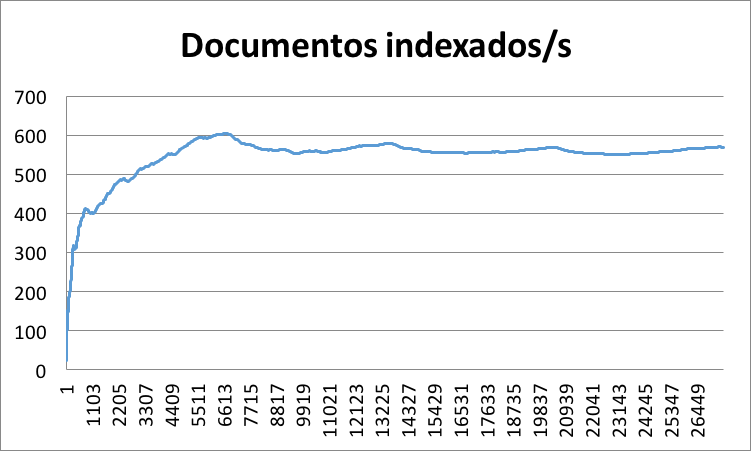
\includegraphics[width=0.6\textwidth]{img/docps}
    \caption{Quantidade de documentos indexados por segundo}
    \label{docs_p_sec}
\end{figure}

\begin{figure}
    \centering
    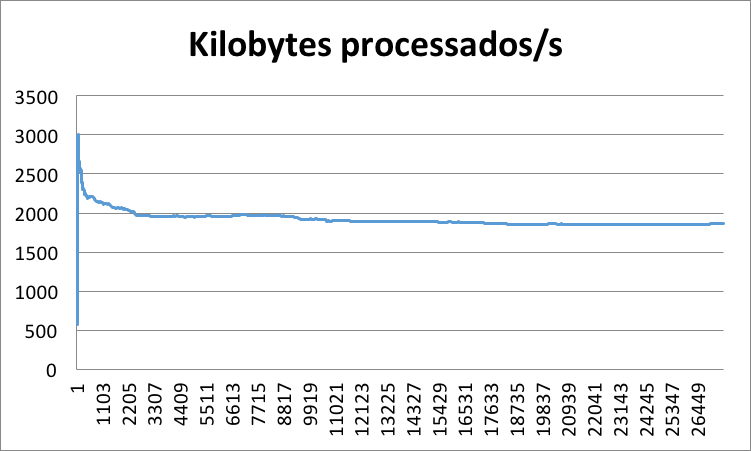
\includegraphics[width=0.6\textwidth]{img/dataps}
    \caption{Quantidade de kilobytes processados por segundo}
    \label{kb_p_sec}
\end{figure}


\subsection{Ranking}

O componente de ranking também é outra adição do Elasticsearch. É possível configurar o fator de similaridade de campos específicos dos documentos, bem como ajustar o valor padrão de todos os campos.

Como mencionado na Seção \ref{ranking}, o modelo de ranking utilizado foi o BM25, com parâmetros \texttt{k1 = 0} e \texttt{b = 0.75}. Acima (Tabela \ref{ranking_table}) estão algumas \emph{queries} e seus devidos valores de precisão e revocação.

\subsection{Interface}

A interface foi implementada seguindo o padrão do protótipo passado, com a exceção de alguns itens, que não puderam ser adicionados e com adição de novos.

Primeiramente a pesquisa é realizada nos campos \texttt{labels} e \texttt{aliases}, podendo ser alterada facilmente para cobrir ``todos os campos''. Essa escolha de implementação foi a que gerou melhores resultados. Os resultados aparecem instantaneamente na tela assim que usuário digita.

\subsubsection{Itens extras}

\begin{itemize}
	\item Mostra imagem quando disponível
	\item Lista com links sociais (website, twitter, etc)
	\item É possível mostrar traduções breves dos títulos e descrições
\end{itemize}

A máquina pode ser acessada através do seguinte endereço:
\hyperref[http://www.cassiano.me/feather]{http://www.cassiano.me/feather}.

\begin{figure}
    \centering
    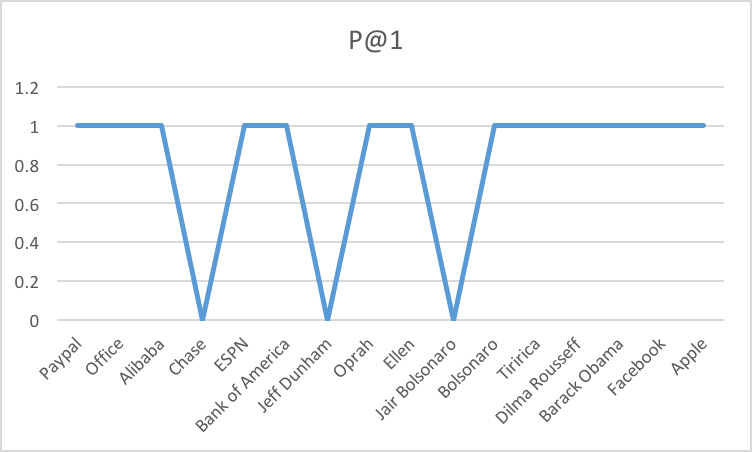
\includegraphics[width=0.6\textwidth]{img/p1}
    \caption{P@1 de consultas do site Alexa.com e do autor}
    \label{interface}
\end{figure}

\begin{table}[]
\centering
\caption{Tabela com pesquisas teste de ranking}
\label{ranking_table}
\begin{tabular}{|l|l|l|l|l|l|}
\hline
Query         & \begin{tabular}[c]{@{}l@{}}\# Docs\\ relevantes\end{tabular} & \begin{tabular}[c]{@{}l@{}}\# Docs\\ retornados\end{tabular} & \begin{tabular}[c]{@{}l@{}}\# Docs relevantes\\ retornados\end{tabular} & Precisão & revocação \\ \hline
Barack Obama  & 8                                                            & 37                                                           & 6                                                                       & 0.22     & 0.75      \\ \hline
Obama         & 11                                                           & 33                                                           & 9                                                                       & 0.33     & 0.81      \\ \hline
Dilma Roussef & 3                                                            & 10                                                           & 3                                                                       & 0.3      & 1         \\ \hline
Brin          & 1                                                            & 3                                                            & 1                                                                       & 0.33     & 1         \\ \hline
\end{tabular}
\end{table}

\section{Conclusão}

Construir um buscador que seja capaz de responder pesquisas com qualidade e em tempo mínimo é uma tarefa árdua e que demanda bastante tempo e conhecimento. Esse trabalho foi uma tentativa de implementar um buscador de entidades seguindo diversas restrições impostas pelo professor.

Em geral, o sistema retorna documentos relevantes em boas posições de ranking. Nos testes realizados, muitas consultas tinham o documento mais relevante (o esperado) em primeiro lugar, mesmo o tamanho da coleção sendo absurdamente grande.

\section{Trabalhos futuros}

Melhorias no sistema de ranqueamento no sentido de adicionar modelos que trabalham com Aprendizado de Máquina podem apresentar melhores resultados, principalmente quando usando \emph{Log} de consultas e recursos externos como os documentos mais vistos ou com mais referências na Wikipedia.

\bibliographystyle{sbc}
\bibliography{sbc-template}

\end{document}
